

\chapter{ شبکه‌های مبتنی بر داده‌های نام‌گذاری شده}
در این فصل به معرفی شبکه‌های مبتنی بر داده‌های نام‌گذاری شده\زیرنوشت{Named Data Networks} می‌پردازیم که ازین به بعد به اختصار آن را  NDN می‌نامیم.  در بخش ابتدایی به بررسی ایرادات شبکه‌های مبتنی بر IP که امروزه به طور گسترده استفاده می‌شوند و در حقیقت زیرساخت شبکه‌های امروزی را تشکیل می‌دهند می‌پردازیم، لزوم روی کار آمدن یک سیستم جدید را نشان می‌دهیم و چشم‌اندازهای آینده برای شبکه‌های NDN را بررسی می‌کنیم. در بخش دوم اساس و پایه‌های طراحی این شبکه‌ها ذکر می‌شود و در نهایت، توضیحات مفصلی راجع به شبکه‌های NDN و چگونگی کارکرد آن‌ها داده می‌شود. 

\section{زمینه و چشم‌انداز}

در دهه‌‌های ۱۹۶۰و ۱۹۷۰ زمانی که پایه‌‌های اینترنت امروزی در حال تبییع شدن بود، ارتباطات در حد ارتباطات تلفنی جهانی تلقی می‌شد. بنابراین راه‌حلی که توسط TCP/IP معرفی شد، مسئله ارتباط نقطه به نقطه\زیرنوشت{point-to-point}بین دو نفر و مکالمه آن‌ها را حل کرد.  
امرزوه شبکه‌ی اینترنت به یک امر فراگیر و همه‌جانبه و حاضر در همه جنبه‌های زندگی روزمره ما تبدیل شده است. در ادامه مصداق‌‌هایی برای این مدعا ذکر می‌کنیم:‌
\شروع{فقرات}
\فقره  تجارت‌های داده محور مانند صنعت گردشگری، بانک‌ها و خدمات اقتصادی مدت‌ها رو به اینترنت آوردند. امروزه تقریبا همه‌چیز به صورت برخط دردسترس است و اینترنت تبدیل به نمایی از جهان شده است. 
\فقره قانون مور که راجع به پیشرفت‌های سخت‌افزاری است، امکان این را فراهم کرده که امروزه همه‌چیز را به اینترنت متصل کنیم. نه فقط ابرکامپیوترها\زیرنوشت{supercomputers} و ایستگاه‌‌های کاری\زیرنوشت{workstations}  بلکه کارخانه‌ها، زیرساخت‌های شهری، تلفن‌ها، اتومبیل‌ها و حتی کلید چراغ‌‌ها. با رشد بی‌وفقه و سریع استفاده از تجهیزات دستی مانند تلفن‌های هوشمند و  تبلت‌ها، تحرک‌پذیری در شبکه اینترنت هم به سرعت رو به افزایش است. 
\فقره امروزه با تبدیل همه انوع فایل از قبیل فایل‌‌های متنی، صوتی، تصویری و ویدئویی به رشته‌های بیتی، و افزایش درخواست برای این محتویات از طرف کاربران، نیاز به مکانیزم قوی‌ای برای توزیع داده روی شبکه اینترنت، بیش از پیش خود را نمایان می‌سازد.
\فقره با امکانات امروزی، هر کاربر به راحتی می‌تواند داده‌های مورد نظر خود را ببیند، از آن‌ها استفاده کند و مهم‌تر از همه خودش محتوا تولید کند. به همین دلیل، سالیانه حجم زیادی از داده تولید و توزیع می‌شود.    
\پایان{فقرات} 

با توجه به تغییرات عمده‌ی ذکر شده، معماری IP ، علی‌‌رغم اینکه برای مکالمه بین دو کاربر نهایی طراحی شده بود، امروزه به صورت گسترده‌ای برای توزیع محتوا مورد استفاده قرار می‌گیرد. هم برای کاربرهای ساکن و هم برای تعداد رو به افزایش کاربران متحرک. همان‌طور که برای توزیع کردن یک خبر، استفاده از رادیو و تلویزیون به مراتب بهینه‌تر از انجام دادن این کار با استفاده از تلفن است،  معماری اینترنت کنونی برای نیازهای امروزی ابزار ضعیفی محسوب می‌شود. علاوه بر این، حملات بدخواهانه، که به دلیل اهمیت بالای داده‌های منتقل شده در اینترنت رو به افزایش هستند، به امری روزمره تبدیل شده‌اند. به دلیل ماهیت مکامله‌ای موجود در ساختار IP ، تلاش‌های بسیاری برای امن‌سازی کانال‌های ارتباطی انجام شده است. ولی با این حال رخنه‌‌های امنیتی با نرخ بالایی در حال افزایش هستند. 

ماهیت مکالمه‌ای حاضر در IP  در شکل داده‌‌ها\زیرنوشت{datagram}ی آن نهفته است. IP فقط نقاط نهایی یک ارتباط را نام‌گذاری می‌کند. در حقیقت در این شبکه‌ها، موجودیت‌های اصلی نقاط انتهایی مکالمه هستند. همان‌طور که از نام NDN مشخص است، هدف این پروژه این است که این محدودیت را برطرف کند و به داده‌ها نام اختصاص دهد. نام‌های داده‌‌ها به صورت  ساختار یافته و سلسه‌مراتبی به آن‌‌ها اختصاص داده می‌شود. همانطور که در TCP/IP ، شناسه ارتباط به همراه عدد توالی یک داده خاص را مشخص می‌کند، در اینجا هم این نام سلسله‌مراتبی داده این کار را انجام می‌دهد. علاوه بر این، مثلا یک قسمت از یک فیلم از شبکه youtube را می‌توان به صورت مستقیم آدرس‌دهی کرد، به جای اینکه مجبور باشیم آن را داخل یک مکالمه بین مشتری و youtube بگنجانیم. این تغییر ساده در معماری IP ، تمرکز را به جای دارندگان داده روی خود اطلاعات می‌گذارد و به همین دلیل داده‌ها را تبدیل به موجودیت‌های اصلی در معماری شبکه می‌کند. 

این تغییر ساده زمینه فرصت‌ها زیادی را فراهم می‌کند:‌
\شروع{فقرات}
\فقره برنامه‌های امروزی بیشتر بر پایه این طراحی شده‌اند که به چه داده‌ای احتیاج دارند نسبت به اینکه این داده را باید از کجا دریافت کنند. امروزه از میان‌افزارهایی استفاده می‌شود که وظیفه نگاشت این داده‌ها به منابع آن‌ها را بر عهده دارند. در مدل NDN ، استفاده مستقیم از برنامه‌ها بدون نیاز به وجود این میان‌افزارها امکان‌پذیر می‌شود.  با حذف این میان‌افزارها، تلاش لازم برای تنظیمات آن‌ها و همچنین نقش غیر بهینه آنها در کارایی برنامه هم حذف می‌شود.  
\فقره در شبکه‌های NDN ،‌ همه داده‌ها توسط تولیدکنندگان آن‌ها امضا شده‌اند و توسط مشتریان اعتبارسنجی می‌شوند. برای مثال در این شبکه‌ها میتوان گواهی داد که همه داده‌ای که یک مشتری در حال دیدن آن است، توسط یک تولیدکننده، تولید و امضا شده است. در حالیکه در شبکه‌های مبتنی بر IP این امکان وجود ندارد. 
\فقره این حقیقت که هر بسته داده مستقل از اینکه از کجا آمده و به کجا می‌رود دارای معنی است، این فرصت را به وجود می‌آورد که در داخل شبکه و مسیریاب‌ها ذخیره شود تا در آینده هم مورد استفاده قرار بگیرد.  همچنین یکتا بودن نام‌های داده‌ها این امکان را فراهم می‌کند تا مسیریاب‌ها بتوانند حالت و وضعیت هر بسته را ذخیره کنند. که این مسئله راه را برای حل بسیاری از مشکلاتی که اینترنت امروزی قادر به رفع آن‌ها نیست هموار می‌کند. یکی از آنها حذف حلقه در مسیر بسته‌هاست. در اینجا هر مسیریاب می‌تواند یک بسته را به تمام واسط‌های خود بفرستد بدون اینکه نگران در حلقه اسیر شدن بسته‌ها باشد. 

\پایان{فقرات}

این تغییر همچنین باعث به وجود آمدن چالش‌هایی هم می‌شود: 
\شروع{فقرات}
\فقره استفاده از نام برنامه‌‌ها برای آدرس‌دهی یک داده در لایه شبکه علاوه بر مزایای ذکر شده در بالا، چالش‌هایی را هم به همراه دارد. از آن جمله می‌توان به این مورد اشاره کرد که یک برنامه چگونه باید داده‌‌های خود را نام‌گذاری کند به نحوی که هم تحویل بسته‌ها در شبکه آسان باشد و هم اینکه با توسعه برنامه، خللی در روند نام‌گذاری ایجاد نشود. 
\فقره مشکل مقیاس‌پذیری در مسیریابی بر اساس داده‌ی نام‌گذاری شده وجود دارد. آدرس‌ها در شبکه‌های IP در یک فضای نام محدود تعریف شده‌اند. درحالیکه در شبکه‌‌های NDN  این فضای نام، بی انتهاست. با این حال، این باور وجود دارد که با استفاده از نام‌گذاری سلسله‌مراتبی، همانند روش که از URL ها برای نام‌گذاری محتوا در اینترنت کنونی استفاده می‌شود می‌توان فضای نام را کنترل کرد همان‌گونه که در شبکه‌های امروزی مسیریاب‌ها از طریق پیشوندهای IP ، آن‌ها را مجتمع می‌کنند. 
\فقره یکی از چالش‌های دیگر مقیاس بزرگ این شبکه‌ها، سرعت در ارسال بسته‌هاست. تحقیقات بسیاری که روی شبکه‌‌های IP انجام شده ثابت‌ کرده‌اند  که می‌توان با استفاده از امکانات سخت‌افزاری، بسته‌ها را با سرعت سیم \زیرنوشت{wire rate}‌ جابجا کرد. انگار که اصلا مسیریابی در بین نبوده است. در واقع این تحقیقات بیان کرده‌اند که وجود مسیریاب‌ها موجب کندی سرعت حرکت بسته‌ها داخل شبکه  نمی‌شود. در مورد شبکه‌های NDN باور بر این است که با استفاده از نتایج تحقیقات گذشته به علاوه مقداری تلاش بیشتر می‌توان به همان سرعت موجود در شبکه‌های IP رسید. 
\پایان{فقرات}

با اینکه NDN یک معماری جدید را معرفی می‌کند، ولی با ساختار اینترنت امروزی سازگار است. لایه‌ی NDN در واقع مانند IP یک پوشش جهانی\زیرنوشت{Universal Overlay} است. NDN می‌تواند روی هر معماری دیگری از جمله IP  اجرا شود. و هر چیز دیگری از جمله IP می‌تواند روی NDN اجرا شود. نکته مثبت این است که زیرساخت‌ها و امکانات ‌IP مانند قرارداد‌های نام‌گذاری DNS\زیرنوشت{Domain Name System} و یا سیاست‌های مسیریابی بین‌دامنه‌ای
\زیرنوشت{inter-domain routing policies} 
که طی دهه‌ها تلاش شکل گرفته‌اند، می‌توانند در NDN هم مورد استفاده قرار بگیرند. از آنجایی که ساختار نام‌‌ها در NDN مشابه ساختار آدرس‌ها در IP و به صورت سلسله‌مراتبی است، الگوریتم‌های موجود در IP می‌توانند با اندکی تغییر در اینجا هم اجرا شوند. 

\section{پایه‌های معماری}
در طراحی معماری شبکه‌های NDN، ۶ پایه درنظر گرفته شده است. ۳ مورد اول پایه‌هایی هستند که از موفقیت سیستم مبتنی بر IP امروزی ناشی می‌شوند و سه مورد آخر ناشی از مسائلی است که گسترش شبکه‌های امروزی آن‌ها را به صورت تجربی اثبات کرده‌اند. 
\begin{itemize}
\item{
\textit{معماری ساعت‌شنی}
 \زیرنوشت{hourglass architecture}
 چیزی است که طراحی اینترنت امروزی را منحصربه‌فرد و قدرت‌مند می‌کند. محوریت این معماری لایه جهانی IP  است که کمینه عملکرد\زیرنوشت{minimal functionality} را برای ارتباطات فراهم کرده است. همچنین این لایه دلیل رشد بدون محدودیت شبکه‌های امروزی است چرا که لایه‌های بالاتر و پایین‌تر مستقل از اینکه چه اتفاقی در لایه شبکه رخ می‌دهد می‌تواند بدون محدودیت گسترش پیدا کنند. همان‌طور که در شکل
~\ref{fig:hourglass}
  مشاهده می‌شود، شبکه‌های NDN هم همین معماری ساعت شنی را استفاده کرده است. 


\begin{figure}[H]
\centering
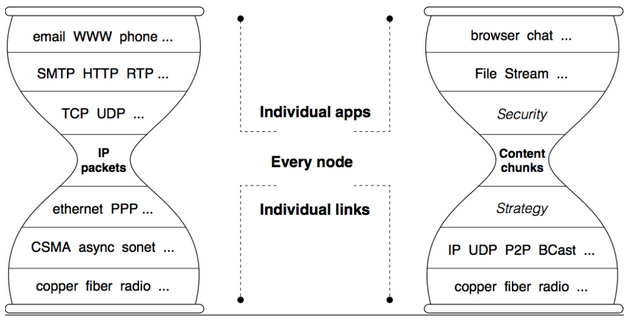
\includegraphics[scale=0.8]{./resources/figures/3_hourglass.png}
\caption{معماری ساعت‌شنی در شبکه‌‌ی اینترنت امروزی و شبکه‌ی NDN}
\label{fig:hourglass}
\end{figure}


%{\begin{figure}[t] \centering \includegraphics[width=#1cm]{resources/figures/#3.png} \caption{#2.} \label{fig:#3} \end{figure}}


} 

\item{
\textit{امنیت}
 یکی از ملزومات طراحی هر معماری‌ای است. امنیت در شبکه‌های امروزی، مسئله‌ای است که بعد از طراحی معماری به آن پرداخته شده است و در واقع در لایه‌های بالاتر و پایین‌تر از لایه شبکه به مسئله امنیت پرداخته شده و در محیط خطرناک اینترنت امروزی، امنیت مورد نیاز را تامین نمی‌کند. امنیت در شبکه‌های NDN یک مسئله پایه‌ای است و برخلاف شبکه‌های IP در همان لایه شبکه به آن پرداخته شده است و با امضا کردن محتوای بسته‌های داده این امنیت را در حد خوبی فراهم کرده است. 

}

\item{
\textit{روش انتها به انتها}
\footnote{end to end principle}
 \cite{end2end}
 که در شبکه‌های امروزی وجود دارد امکان مقابله در صورت بروز مشکل در شبکه  را فراهم می‌کند. اگر از روش انتها به انتها استفاده کنیم، در صورت از کار افتادن یکی از پیوندهای موجود در شبکه، از‌آنجایی که فقط به مقصد رسیدن بسته مهم است، مسیریاب\زیرنوشت{router} می‌تواند بسته را از یک مسیر دیگر بفرستد و بسته در نهایت به مقصد خود می‌رسد ولی در صورتی که اگر از روش نقطه به نقطه\زیرنوشت{point to point principle} استفاده شده باشد، در صورت بروز چنین رخدادی، بسته در میانه‌ی راه رها می‌شود. این رویه در شبکه‌های NDN هم وجود دارد. 
}

\item{
\textit{ترافیک شبکه}
باید به نحوی باشد که بتواند خودش را با تغییرات تطبیق دهد. جریان معتدل داده‌ها در داخل شبکه برای داشتن یک شبکه پایدار ضروری است. در سیستم مبتنی بر IP ، چون امکان به وجود آمدن حلقه در رسیدن بسته‌ها به مقصد وجود دارد، پروتکل‌های لایه انتقال هستند که در مقابل رویداد چنین وقایعی ارتقا داده شده‌اند. ولی در شبکه‌‌های NDN، در همان لایه شبکه مکانیزمی برای مقابله با به وجود آمدن حلقه در نظر گرفته شده است. 
}
\item{
\textit{جدا بودن دامنه مسیریابی و ارسال}
\footnote{forwarding}
یکی از مسائلی است که ثابت شده برای توسعه اینترنت امری ضروری است. فایده این کار این است که سیستم ارسال می‌تواند به کار خود ادامه دهد درحالیکه سیستم مسیریابی به صورت مستقل خودش را با تغییرات شبکه تطبیق می‌دهد.  معماری حاکم بر NDN هم همین رویه را پیش‌رو گرفته و امکان مستقل کار کردن این دو دامنه را فراهم کرده است. 
}

\item{
\textit{ معماری باید انتخاب کاربر و رقابت را در مواقع امکان‌پذیر فراهم کند }
هرچند که این فاکتور، در طراحی معماری اصلی اینترنت جایگاهی نداشته است، ولی گسترش شبکه‌ها این قضیه را اثبات کرده است که معماری نباید نقش خنثی‌ای داشته باشد. معماری NDN تلاش آگاهانه‌ای در جهت قدرتمند کردن کاربران نهایی و همچنین به وجود آمدن رقابت کرده است. 
\cite{clark2002tussle}
}

\end{itemize}

\section{معماری NDN}
مشابه شبکه‌های مبتنی بر IP، محوریت معماری شبکه‌های NDN  نیز همان میانه ساعت شنی ذکر شده در قسمت قبل است. ولی در این شبکه‌ها از داده‌‌های نام‌گذاری شده به جای آدرس‌های IP استفاده می‌‌شود. این تغییر علی‌رغم سادگی‌اش، موجب به وجود آمدن تفاوت‌های زیادی بین عملکرد این شبکه‌ها در رساندن بسته‌ها با شبکه‌های پیشین که مبتنی بر IP بودند، شده است.  در این بخش ابتدا یک توضیح مختصر راجع به مفاهیم کلی در شبکه‌های NDN داده می‌شود و سپس راجع به هر عنصر و هم‌چنین نقش آن در معماری کلی به تفضیل صحبت می‌شود. 

\begin{figure}[H]
\centering
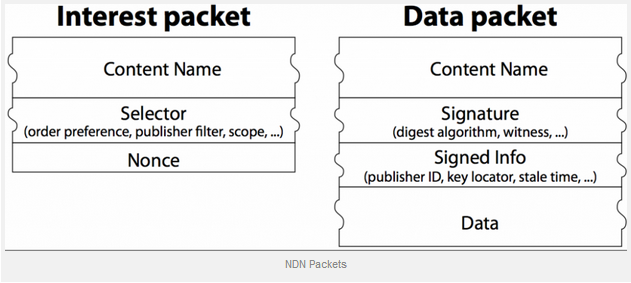
\includegraphics[scale=0.75]{./resources/figures/3_NDNpackets.png}
\caption{بسته‌ها در معماری NDN}
\label{fig:packets}
\end{figure}

\begin{figure}[H]
\centering
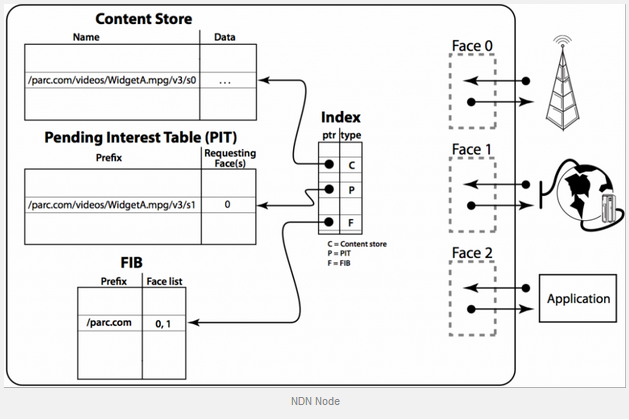
\includegraphics[scale=1]{./resources/figures/3_NDNnode.png}
\caption{ساختار یک مسیریاب در شبکه‌های مبتنی بر داده‌ی نام‌گذاری‌شده}
\label{fig:node}
\end{figure}



ارتباطات در شبکه‌های NDN بر پایه درخواست یک مشتری آغاز می‌شود. مشتری برای اینکه به داده‌ای دسترسی پیدا کند، یک بسته از نوع درخواست\زیرنوشت{interest packet} می‌فرستد که شامل یک نام است که ماهیت داده مورد نظر را مشخص می‌کند (شکل
‍‍‍‍~\ref{fig:packets}
). مسیریاب واسطی\زیرنوشت{interface} که این بسته از آن رسیده است را به خاطر می‌سپارد و بعد این بسته را بر پایه داده‌های \مهم{جدول اطلاعات ارسال}\زیرنوشت{Forwarding Informaion Base} (FIB) بر روی واسط درست ارسال می‌کند. این جدول به وسیله نتایج حاصل از کارکرد پروتکل مسیریابی به روزرسانی می‌شود. وقتی که بسته درخواست به گره‌ای رسید که حاوی اطلاعات موردنظر بود، یک بسته داده\زیرنوشت{data packet} فرستاده می‌شود. که شامل نام و محتوایات داده است که به وسیله گره ارسال کننده اطلاعات امضا شده‌اند. مسیری که توسط بسته داده طی می‌شود تا به دست مشتری برسد، دقیقا برعکس مسیری است که بسته درخواست طی کرده است. لازم به ذکر است که هیچ‌کدام از بسته‌‌های درخواست و یا داده شامل هیچ آدرس میزبان و یا واسطی نظیر آنچه در IP  داریم، نیستند. بسته‌های درخواست براساس نامی که در آن‌ها ذکر شده است، به سمت مقصد خود روانه می‌شوند و بسته‌های داده هم بر اساس اطلاعات نگه‌داری شده در هر گره بین راه حرکت می‌کنند تا به دست مشتری برسند. (‌شکل
~\ref{fig:node}
)

مسیریاب‌ها تمام درخواست‌‌هایی که منتظرند تا بسته داده آن‌ها برسد را در جدولی به نام جدول درخواست‌های معلق\زیرنوشت{Pending Interest Table}
(PIT)
ذخیره‌ می‌کنند. وقتی که درخواست‌‌‌های متعددی برای یک داده به یک مسیریاب می‌رسد، فقط اولین درخواست به سمت منبع داده مورد نظر ارسال می‌شود. هر سطر جدول PIT شامل یک نام و همچنین تمام واسط‌‌هایی است که حداقل یک بسته درخواست برای این داده از طریق آن‌ها دریافت شده است. وقتی که یک بسته داده به مسیریاب می‌رسد، مسیریاب سطر مربوطه را از جدول ذخیره‌شده بازیابی می‌کند و بسته داده را به تمام واسط‌هایی که برای این داده ثبت شده بودند، ارسال می‌کند. سپس سطر مربوطه را از جدول PIT  حذف می‌کند و در ادامه، بسته داده را در بانک داده‌\زیرنوشت{Content Store}ی خود ذخیره‌سازی می‌کند. از آنجایی که یک بسته داده در شبکه‌های NDN مستقل از آنکه از کجا آمده و به کجا می‌رود، بامعنا است، مسیریاب‌ها می‌توانند آن‌ها را ذخیره کنند تا در موارد آینده که درخواست این داده به آن‌ها می‌رسد، به این درخواست پاسخ بگویند. 

\subsection{نام‌گذاری}
طراحی شبکه‌های NDN بر پایه‌ی نام‌گذاری‌های سلسله‌مراتبی و ساخت‌یافته‌ی\زیرنوشت{hierarchically structured names} داده‌ها است. برای مثال یک فیلم که شرکت سازنده‌ی آن PARC است، می‌تواند نام /parc/videos/WidgetA.mpg را داشته باشد. علامت / مشخص‌کننده مرز بین مولفه‌ها است و جزئی از نام محسوب نمی‌شود. این ساختار سلسله‌مراتبی به برنامه‌های این امکان را می‌دهد که روابط بین داده‌های مختلف را نمایش دهند. برای مثال، نام بخش ۳ از نسخه ۱ این فیلم می‌تواند /parc/videos/WidgetA.mpg/1/3 باشد. این ساختار همچنین باعث می‌شود که مسیریابی مقیاس‌پذیر شود. هرچند به صورت تئوری ممکن است که مسیریابی بر اساس نام‌های تخت\زیرنوشت{flat names}  هم صورت پذیرد،
\cite{rofl}
 ولی این ساختار سلسله‌مراتبی است که امکان تجمع را فراهم می‌کند که در مبحث مسیریابی امری ضروری برای مقیاس‌پذیری محسوب می‌شود. ساختارهایی که برای ارتباط در این شبکه لازم است توسط قرارداد‌هایی بین مشتری و تولیدکننده‌ی محتوا تعیین می‌شود. برای مثال قراردادهایی برای درنظر گرفتن نسخه و بخش‌های یک فیلم.
 
قراردادهایی که برای نام‌گذاری وجود دارند، برای برنامه‌ها قابل فهم‌اند ولی از دید شبکه معنی‌ای ندارند.\زیرنوشت{opaque} یک مسیریاب نمی‌داند که منظور از نام یک داده خاص چیست، هرچند که قسمت‌های مختلف آن را که از هم جدا شده‌اند می‌بیند. این موضوعِ، به برنامه‌ها این قابلیت را می‌دهد که روش نام‌گذاری خاص خود را با توجه به نیاز‌های خود و مستقل از بقیه نام‌گذاری‌ها داشته باشند. 

برای بازیابی داده‌هایی که به صورت پویا تولید می‌شوند، مشتری باید بتواند که نام داده‌ی موردنظر خود را به صورت قطعی\زیرنوشت{deterministically } تعیین کند، بدون آنکه از قبل آن را دیده باشد. برای این مسئله دو راهکار وجود دارد. یکی اینکه یک الگوریتم قطعی برای تعیین نام داده‌ها بین مشتری و تولیدکننده وجود داشته باشد  و دیگری اینکه مشتری می‌تواند نام داده را از نام ناقصی که از تولیدکننده دریافت‌ می‌کند، استخراج کند. برای مثال مشتری /parc/videos/WidgetA.mpg را درخواست می‌کند و یک بسته داده با نام  parc/videos/WidgetA.mpg/1/1 دریافت می‌کند. زین پس، مشتری می‌تواند قسمت‌های بعدی را با ترکیب قوانین قرارداد موجود و اطلاعاتی که از روی اولین بسته دریافت‌شده بدست می‌آورد، تعیین کند و آنها را از تولیدکننده درخواست نماید. 

نیازی نیست که همه اسامی به صورت سراسری یکتا باشند. تنها آن بسته‌هایی که حاوی اطلاعاتی هستند که به صورت سراسری مورد استفاده قرار می‌گیرند باید دارای نام‌های یکتا باشند. نام‌‌هایی که برای ارتباطات محلی به کار گرفته می‌شوند ممکن است که وابسته به داده‌های همان شبکه باشند و انتقال این اطلاعات فقط با ارتباطات محلی صورت می‌پذیرد. حتی استفاده از نام‌های منحصربه‌فرد می‌تواند در دامنه‌ها و مواقع خاصی مفید هم واقع شود. حتی نامی مانند «وضعیت روشنایی چراغ داخل سالن» می‌تواند یک نام باشد. پیدا کردن راهبردهای جدیدی که هر داده را با توجه به دامنه‌ای که در ‌آن معنا دارد بررسی کند، یک مسئله پژوهشی جدید است. 

مدیریت فضای نام جزئی از معماری شبکه‌های NDN  محسوب نمی‌شود، همان‌طور که شبکه‌های مبتنی بر IP از IP استفاده می‌کنند ولی مدیریت اختصاص IP جزو معماری این شبکه محسوب نمی‌شود. با این حال، نام‌گذاری داده‌‌ها، مهم‌ترین بخش طراحی معماری NDN است. داده‌های نام‌گذاری‌شده این قابلیت را به NDN می‌دهد که به صورت خودکار کارایی‌های زیادی را پشتیبانی کند. از آن جمله می‌توان به موارد زیر اشاره کرد:
\شروع{فقرات}
\فقره \مهم{توزیع محتوا}\زیرنوشت{content distribution}: کاربران مختلفی در مواقع مختلف یک داده را درخواست می‌کنند. 
\فقره \مهم{چندپخشی}\زیرنوشت{multicast}: کاربران مختلفی یک داده را در یک زمان درخواست می‌کنند.
\فقره \مهم{پویایی}\زیرنوشت{mobility}:‌  به دلیل عدم وابستگی ارتباط به مکان داده، کاربران می‌توانند داده‌ها را از مکان‌های متفاوتی درخواست کنند. 
\فقره \مهم{تحمل‌پذیری تاخیر}\زیرنوشت{delay-tolerant networking}: به دلیل عدم وابستگی ارتباط به مکان داده، شبکه‌های DTN بر پایه NDN به خوبی قابل پیاده‌سازی هستند. 
\پایان{فقرات}

تحقیقات راجع به اینکه بهترین نحوه نام‌گذاری داده‌ها چگونه است و تلاش در راستای تبیین کردن قوانینی برای نام‌گذاری به صورت سراسری همچنان ادامه دارد. فایده وجود چنین قوانینی این است که استفاده مجدد داده‌ها در آینده را امکان‌پذیر می‌کند.  
\subsection{امنیت داده‌محور}
در شبکه‌های ‌NDN ، امنیت در بسته داده تعبیه شده است. به جای آنکه تابعی از این باشد که این بسته چگونه و از کجا به دست آمده است. 
\cite{nnt}
هر بسته داده‌ای همراه با نام آن امضا شده است. امضا کردن داده‌‌ها اجباری است و هیچ برنامه‌ای نمی‌تواند داده‌ی غیرامضا شده بفرستد. اطلاعات استخراج شده از  امضا و اطلاعات منتشرکننده‌ی بسته‌ی داده، این امکان را فراهم می‌کند تا مشتری بتواند منشا داده را تشخیص دهد. همچنین این رویه باعث می‌شود که  اعتماد مشتری به صحت داده از اینکه داده چگونه و از چه مسیری به دست او رسیده مستقل باشد. همچنین از دیگر فایده‌های این رویه این است که اعتماد به صورت ریزدانه است. به این معنی که مشتری می‌تواند با بررسی کلید عمومی یک منتشرکننده تصمیم بگیرد که آیا این منتشرکننده را، منبع امنی برای یک داده خاص در یک زمینه خاص می‌شناسد یا خیر. به بیان دیگر لازم نیست که به یک منتشر کننده به صورت کامل اعتماد داشته باشیم یا نداشته باشیم. بلکه می‌توانیم با توجه به داده‌ها تصمیم بگیریم که آیا به یک منتشرکننده اعتماد داریم یا خیر. 
 
 از طرف دیگر پیاده‌سازی این اعتماد ریزدانه و همچنین امنیت داده‌محور به صورت عملی، نیازمند خلاقیت است.  تچربه ثابت کرده است که رمزنگاری بر پایه کلید عمومی و خصوصی از کارایی لازم برخوردار نیست و همین‌طور پیاده‌سازی آن دشوار است. در کنار امضاهای دیجیتال کارا، NDN نیاز به یک روش قابل انتعطاف و کارا برای مدیریت اعتماد کاربران دارد. از‌ آنجایی که کلیدها می‌توانند به عنوان داده رد و بدل شوند، توزیع کلید کار آسانی است. 
یک مبنا برای بسیاری از مدل‌های اعتماد، مقید کردن نام‌ها به داده‌ها  است. برای مثال اگر داده، یک کلید عمومی است،  این مقید کردن، یک گواهی کلید عمومی است. در آخر، طراحی انتها به انتها در NDN، امکان اعتمادسنجی درست را بین مشتریان وتولیدکنندگاه فراهم می‌کند. این مدل به تولیدکنندگان و مشتریان این انعطاف‌پذیری را می‌دهد که مدل‌های اعتمادی خود را به دلخواه خود انتخاب کنند. 


\subsection{مسیریابی و ارسال}
در شبکه‌های NDN، کار مسیریابی و ارسال بسته‌ها بر اساس نام آن‌ها انجام می‌شود. این کار باعث می‌شود تا چهار مشکلی که در معماری IP وجود داشت، مرتفع گردد:‌ 
\شروع{فقرات}
\فقره \مهم{تمام شدن فضای آدرس}\زیرنوشت{address space exhaustion}. فضای آدرس در شبکه‌های NDN تمام نمی‌شود چون هیچ محدودیتی برای نام‌گذاری نداریم و نامتناهی می‌توانیم داده با نام‌های مختلف داشته باشیم. 
\فقره \مهم{
پیمایش\زیرنوشت{Traversal}
NAT \footnote{Network Address Translation}
} 
مشکلی که در NAT وجود دارد این است که امکان ارتباط با سرور از پشت یک شبکه NAT وجود ندارد. در شبکه‌های NDN از آنجایی که میزبان نیازی به اعلام آدرس خود برای اعلام داده‌هایی که ذخیره کرده است ندارد، این مشکل وجود ندارد.  
\فقره \مهم{تحرک‌پذیری}\زیرنوشت{mobility}: متحرک بودن عوامل، در شبکه‌های IP نیازمند تغییر IP است ولی در شبکه‌های NDN، دیگر ارتباطات به دلیل تحرک عوامل قطع نمی‌شوند چون اسامی داده‌ها همیشه ثابت‌اند. 
\فقره \مهم{مدیریت فضای آدرس}:‌ مدیریت و تخصیص آدرس در شبکه‌های مبتنی بر IP یک چالش محسوب می‌شود ولی در این شبکه‌ها این مشکل برطرف شده است. 
\پایان{فقرات}

پروتکل‌های مسیریابی تست‌شده و معتبری مثل BGP\footnote{Border Gateway Protocol} ،
IS-IS\footnote{Intermediate System to Intermediate System}و 
OSPF\footnote{Open Shortest Path First}
که در شبکه‌های مبتنی بر IP وجود دارند، را می‌توان با تغییرات اندکی در این شبکه‌ها هم استفاده کرد. به جای اعلام کردن پیشوندهای IP، یک مسیریاب NDN، باید پیشوندهای نام‌هایی را اعلام کند که داده مربوط به آن‌ها را در اختیار دارد. 
این اعلام به وسیله پروتکل مسیریابی در در سرتاسر شبکه پخش می‌شود و هر مسیریاب جدول FIB خود را بر اساس اطلاعات دریافتی به روزرسانی می‌کند. هرچند، نامتناهی بودن فضای نام‌ها این سوال را پیش می‌آورد که چگونه اندازه جدول مسیریابی در حد معقولی باقی بماند. 

مسیریاب‌ها با نام‌‌های داده‌‌ها همانند یک دنباله از مولفه‌های مبهم\زیرنوشت{opaque} برخورد می‌کنند و برای هر بسته در جدول FIB به دنبال سطری می‌گردند که بلندترین پیشوند مشترک را با نام بسته موردنظر داشته باشد. برای مثال، بسته‌ای با نام /parc/videos/WidgetA.mpg می‌تواند هم با /parc/videos منطبق شود و هم با /parc ولی اولی به عنوان جواب جستجو برگردانده می‌شود.  این سوال مطرح است که آیا جستجوی در جدولی که حاوی نام‌های غیرهم‌طول و همچنین سلسله‌مراتبی است می‌تواند در زمان خطی انجام پذیرد یا خیر. 

NDN
 به طور ذاتی مسیریابی چندمسیری را پشتیبانی می‌کند. مسیریابی IP به این صورت است که برای جلوگیری از رخداد حلقه، بهترین مسیر انتخاب می‌شود و بسته فقط از طریق یک واسط فرستاده می‌شود. در شبکه‌های ‌NDN، بسته‌های درخواست نمی‌توانند در داخل حلقه بیفتند چون به همراه هر نام، یک نانس هم فرستاده می‌شود که با استفاده از آن می‌توان تکراری بودن بسته را مشخص کرد. به این صورت که هر مسیریاب در داخل جدول PIT  خود، این نانس‌ها را هم ذخیره می‌کند و هربار که یک بسته به مسیریاب رسید، نانس آن با نانس همه بسته‌‌های هم‌نام آن که در داخل PIT  ذخیره شده بودند، مقایسه می‌شود و در صورت تکراری بودن، بسته رسیده شده در نظر گرفته نمی‌شود. بسته‌های داده هم نمی‌توانند در داخل حلقه بیفتند چرا که مسیر آن‌ها دقیقا برعکس مسیر طی‌شده توسط بسته درخواست مربوطه است. به همین دلیل، یک مسیریاب بدون آنکه نگران ایجاد حلقه در مسیر بسته‌ای باشد، می‌تواند یک بسته را روی چندین واسط خود ارسال کند. اولین جوابی که از راه می‌رسد، همه درخواست‌ها برای آن داده را ارضا می‌کند و به صورت محلی ذخیره می‌شود و جواب‌های بعدی همه به دور انداخته می‌شوند. 
این قابلیت چندمسیری در شبکه‌های NDN، باعث می‌شود که توازن بار متعادلی در داخل شبکه به وجود بیاید. همین‌طور انتخاب و اولویت‌بندی مسیرها را امکان‌پذیر می‌کند. به این صورت که یک مسیریاب چندین بسته اول را روی همه واسط‌های ممکن ارسال می‌کند، سپس کارایی هر واسط را با توجه به زمان برگشت جواب از آن واسط محاسبه می‌کند و بر اساس این داده‌ها، بهترین مسیر(ها) را برای درخواست‌های آینده برای آن داده خاص محاسبه ‌می‌کند.به الگوریتم‌هایی که وظیفه این محاسبات را بر عهده دارند، راهبرد ارسال\زیرنوشت{Forwarding Strategy} گفته می‌شود. 


NDN
می‌تواند امنیت مسیریابی را به شدت افزایش دهد. اول از همه، امضا کردن همه داده‌‌ها، به خصوص  پیام‌های مسیریابی، از دستکاری پیام‌ها جلوگیری می‌کند. از طرف دیگر، پشتیبانی از امکان چندمسیری\زیرنوشت{multipath}  به همراه دامنه‌ی داده‌ی هوشمند\زیرنوشت{Intelligent Data Plane}(که در قسمت بعد در مورد آن توضیح می‌دهیم)، می‌توانند در کاهش ربایش پیشوندها\زیرنوشت{Prefix Hijacking} نقش به‌سزایی را ایفا کنند. چرا که مسیریاب‌ها می‌توانند ناهنجاری حاصله از ربایش پیشوندها را شناسایی کنند و اطلاعات اصلی و درست را از طرق دیگر بدست بیاورند. در نهایت، این حقیقت که پیام‌های NDN  فقط راجع به داده هستند و هیچ اطلاعاتی را از میزبان حمل نمی‌کنند، باعث می‌شود که فرستادن بسته‌‌های مخرب با هدف اینکه به مکان خاصی برسند، کار سختی باشد. 
حملات بر ضد NDN ، اگر بخواهند که موثر واقع شوند، باید تمرکز خود را بر روی منع سرویس بگذارند. مشکلی که هم‌اکنون تحقیقات زیادی برای رفع آن در حال انجام است. 

 
\subsection{دامنه داده هوشمند}
در دامنه داده، جدول PIT همه درخواست‌های معلق را که هنوز جواب آن‌ها نرسیده را در خود ذخیره می‌کند. هر سطر این جدول شامل یک نام و واسط‌هایی که این داده را درخواست کرده‌اند. در صورتی که داده مربوط به یک درخواست بیاید و یا اینکه زمان انتظار به پایان برسد، آن سطر از داخل جدول حذف می‌شود. این رویه که به ازای هر بسته یک حالت ذخیره می‌شود، یک تغییر بنیادی نسبت به شبکه‌های IP محسوب می‌شود، جایی که دامنه داده، حالتی ندارد. \زیرنوشت{Stateless}   . این حالت‌دار بودن دامنه داده در شبکه‌های NDN، این شبکه‌ها را به شبکه‌هایی سازگار در مقابل شکست‌های شبکه تبدیل می‌کند و همچنین باعث می‌شود که در استفاده از منابع شبکه کارایی بالایی داشته باشیم. در ادامه درباره این حالت‌دار بودن وضعیت توضیح بیشتری می‌دهیم. 

 یک گره در شبکه NDN  می‌تواند بر اساس جدول PIT و بسته‌ی داده رسیده شده (‌و یا اتمام وقت انتظار) ،  بر عملکرد واسط‌های مختلف در راستای رساندن پیام‌ها نظارت داشته باشد. و همچنین گم شدن بسته‌ها را شناسایی و کشف کند. حاصل این نظارت، تبیین معیاری به اسم زمان رفت‌وبرگشت\زیرنوشت{round-trip time} است  بر اساس جدول PIT  و یک عدد نانس که به همراه هر بسته درخواستی فرستاده می‌شود، اگر یک بسته برای بار دوم به یک گره برسد به آسانی شناسایی می‌شود و به دور انداخته می‌شود. همان‌طور که در قسمت قبل توضیح داده‌ شد، مسیریاب‌ها با تصمیم‌گیری روی اینکه یک داده را روی کدام واسط بفرستند باعث متعادل شدن بار درون شبکه می‌شوند و همچنین در صورت خرابی پیوندهای شبکه، آن‌ها را شناسایی می‌کنند و از مسیرهای دیگر داده درخواست شده را به دست می‌آورند. 
 
وجود جدول PIT  در هر مسیریاب اهداف مهم دیگری را هم برآورده می‌کند. از آنجایی که این جدول برای هر داده، همه واسط‌هایی که این داده را درخواست کرده‌اند را نگه‌داری می‌کند، در حقیقت پتانسیل چندپخشی را به معماری عطا می‌کند. چرا که وقتی داده مورد نظر از یکی از واسط‌ها رسید، این بسته به همه واسط‌هایی که طالب این داده بودند، ارسال می‌شود. در واقع با انجام این عمل، مسیریاب نقش موثری در کاهش بار شبکه ایفا می‌کند. همچنین از آنجایی که به ازای هر بسته درخواست یک بسته داده وجود دارد، مسیریاب با کنترل کردن تعداد بسته‌های درخواست معلق می‌تواند تعادل جریان داده را در درون شبکه به وجود بیاورد.  از مزایای دیگر وجود جدول PIT می‌توان به کاهش احتمال حمله منع سرویس\زیرنوشت{Distributed denial-of-service attack} 
(DDoS )
 اشاره کرد. از آنجایی که تعداد سطر‌های جدول PIT  معیار خوبی برای مقدار باری است که روی شبکه وارد شده است، در نظر گرفتن یک حد بالا برای آن، میزان تاثیرپذیری در مقابل حمله DDoS را تعیین می‌کند. زمان انتظار هر عضو از جدول PIT ، در مقابله با حملات مفید‌اند زیرا که بعد از مدت زمانی داده از جدول حذف می‌شود و مانع از بیش از اندازه بزرگ شدن جدول می‌شود.
\cite{lads}
در نهایت اطلاعات بدست آمده از واسطی که داده مورد نظر از طریق آن رسیده، داده‌هایی را فراهم می‌کند که با کمک آن‌‌ها میتوان برای  پیاده‌سازی یک شمای پس‌زدن\زیرنوشت{push-back scheme}
\cite{pushback}
 از آن استفاده کرد. 
\subsection{ذخیره‌سازی}
داده‌های نام‌گذاری شده، امکان ذخیره‌سازی درون‌شبکه‌ای خودکار را فراهم‌ می‌کنند. از آنجایی که هر بسته داده در NDN مستقلا از این که از کجا آمده و به کجا می‌رود با معنی است، مسیریاب‌ها می‌توانند آن‌ها را در بانک داده خود ذخیره کنند تا در آینده از آنها استفاده کنند. زمانی که یک درخواست جدید به یک مسیریاب می‌رسد، مسیریاب ابتدا بانک داده خود را جستجو می‌کند، اگر داده‌ای هم‌نام با داده‌ي درخواست شده پیدا کند، آن داده را به عنوان جواب برمی‌گرداند. بانک داده در حقیقت نقش همان حافظه‌‌ی میان‌گیر\زیرنوشت{memory buffer} در مسیریاب‌های امروزی را ایفا می‌کند. هردوی آن‌ها بسته‌‌های داده را ذخیره‌ می‌کنند. تفاوت آن‌ها این است که مسیریاب‌‌های IP بعد از ارسال نمی‌توانند از آن‌ها استفاده کنند ولی مسیریاب‌های NDN  می‌توانند از آن‌ها استفاده مجدد بکنند چرا که داده‌‌ها فقط با استفاده از نامشان از همدیگر متمایز می‌شوند. در مورد داده‌های ایستا، NDN تقریبا به بهینه‌ترین حالت برای رساندن پیام‌ها رسیده است. چرا که مثلا چند نفر که به طور همزمان یک URL را وارد می‌کنند و می‌خواهند محتویات یک سایت را ببینند، برخلاف رویه‌ای که در شبکه IP وجود دارد، تک تک درخواست‌های آن‌ها به سرور نمی‌رسد و هرکدام جداگانه یک جواب از سرور دریافت نمی‌کنند. بلکه بعد از اینکه جواب اولین درخواست از طرف سرور رسید، در مسیریاب اول ذخیره می‌شود و از آن به بعد هر کسی که درخواست ورود به همان سایت را داشت، همان مسیریاب اول به او پاسخ می‌گوید و نیازی نیست که هر درخواستی دوباره تا سرور برود و برگردد. حتی در مورد محتویاتی که به صورت پویا تولید می‌شوند هم NDN از کارایی بالایی برخوردار است. برای مثال در یک جلسات برخط ویدیویی که داده باید به دست چندین نفر برسد، و یا ارسال مجدد بسته‌ها در مواقعی گم شدن بسته‌ها. (مراجعه کنید به بخش 
\ref{section:enteghal}
) که در این شرایط هم ذخیره‌سازی داده‌ها در بانک داده مسیریاب‌ها می‌تواند مثمر ثمر واقع شود. 

ذخیره‌سازی داده‌های نام‌گذاری شده ممکن است موجب به وجود آمدن مسائل امنیتی شود. شبکه IP امروزی از ضعف حفاظت امنیتی رنج می‌برد. به طور پیش‌فرض (و بدون در نظر گرفتن ملاحظات امنیتی که امروزه در لایه‌هایی به جز لایه شبکه اعمال می‌شوند) یک مهاجم می‌توانند با دیدن سرآیند و یا بخش داده‌ای یک بسته بفهمد که محتویات یک بسته چیست و با مشاهده آدرس‌های مبدا و مقصد بسته می‌تواند بفهمد که چه‌کسی این داده را درخواست کرده است. در NDN، داده‌ها نام‌گذاری شده‌اند و کسی که  ناظر شبکه است، به راحتی می‌تواند بفهمد که چه داده‌ای درخواست شده است. مهاجم می‌تواند با کاوش و رصد دقیق بسته‌ها بفهمد که چه داده‌هایی داخل بانک داده مسیریاب ذخیره شده‌اند ولی هیچ اطلاعاتی راجع به اینکه چه کسی این داده را درخواست کرده است نمی‌تواند بدست بیاورد. به دلایلی که ذکر شد، شبکه‌های NDN امنیت را به طور کلی در یک سطح دیگری نسبت به آنچه در IP  داریم تامین کرده‌اند. 


\subsection{انتقال}
\label{section:enteghal}
معماری NDN  دارای یک لایه انتقال جداگانه نیست. در این معماری، کارکردهای لایه انتقال به لایه کاربر\زیرنوشت{application layer}، کتابخانه‌های پشتیبان و مولفه‌‌های راهبردی در دامنه ارسال منتقل شده است. تسهیم\زیرنوشت{Multiplexing} و عدم تسهیم\زیرنوشت{Demultiplexing} در بین فرایندهای برنامه‌ها به طور مستقیم توسط لایه NDN انجام می‌شود و جامعیت داده‌ها و قابلیت اطمینان به وسیله فرایندهای کاربر از قبیل بررسی درجه اطمینان، امضای داده‌ها و تصمیمات اعتمادی مدیریت می‌شود. 
مسیریاب‌‌های ‌NDN، ترافیک شبکه را با تعیین نرخ ارسال بسته‌های درخواست مدیریت می‌کنند.  وقتی حجم زیادیی از بسته‌های داده از طریق یک همسایه به یک مسیریاب می‌رسد، آن مسیریاب به سادگی نرخ فرستادن بسته‌های درخواست به آن همسایه را کاهش می‌دهد و یا قطع می‌کند. این به این معنی است که NDN وظیفه کنترل ازدحام\زیرنوشت{Congestion Control} را از دوش کاربران نهایی برداشته است. وقتی که ازدحام رخ می‌دهد، ذخیره‌سازی داده‌ها، کار بازارسال بسته‌ها را تسهیل می‌کند. چرا که نیازی نیست که بسته دوباره از مبدا فرستاده شود بلکه از آخرین جایی که قبل از آن بسته گم شده بود فرستاده می‌شود. این مسئله وقتی بیشتر به چشم می‌آید که مثلا بسته در پیوندهای آخر گم می‌شود و در شبکه‌‌های IP مجبور است که کل مسیر را دوباره طی کند و موجب شلوغی و سربار روی شبکه می‌شود ولی در اینجا تنها همان پیوند آخر را دوباره پیمایش می‌کند.   


